\PassOptionsToPackage{unicode,pdfusetitle}{hyperref}
\PassOptionsToPackage{hyphens}{url}
\PassOptionsToPackage{dvipsnames,svgnames,x11names}{xcolor}

\documentclass[aspectratio=1610,onlytextwidth]{beamer}

\usetheme{moloch}
\usefonttheme{professionalfonts}
\setbeamertemplate{page number in head/foot}[appendixframenumber]

\usepackage{listings}
\usepackage{lstautogobble}
\lstset{
  autogobble,
  language=R,
  showspaces = false,
  morekeywords={TRUE, FALSE},
  showtabs = false,
  breaklines = true,
  tabsize = 2,
  keywordstyle=\color{SteelBlue4},
  stringstyle=\color{RedViolet},
  deletekeywords={data,frame,length,as,character},
  basicstyle=\ttfamily\footnotesize
}

\usepackage{lmodern}
\usepackage{amssymb,amsmath,mathtools,amsthm}
\usepackage[T1]{fontenc}
\usepackage{textcomp}

% \usepackage{minted}

\usepackage{upquote} % straight quotes in verbatim environments
\usepackage{microtype}
\UseMicrotypeSet[protrusion]{basicmath} % disable protrusion for tt fonts

\usepackage{xcolor}
\usepackage{xurl} % add URL line breaks if available
\usepackage{bookmark}
\usepackage{hyperref}

\usepackage{tikz}

\hypersetup{%
  colorlinks = true,
  linkcolor  = mLightGreen,
  filecolor  = mLightGreen,
  citecolor  = mLightGreen,
  urlcolor   = mLightGreen
}

% animations
\usepackage{xmpmulti}

%% subfigures
% \usepackage{subcaption}

% algorithms
\usepackage[ruled,vlined]{algorithm2e}
\resetcounteronoverlays{algocf}

\usepackage{booktabs}

\date{\today}
\titlegraphic{\hfill
\includegraphics[width=4cm]{images/ucph-horizontal-right.pdf}\vspace{1cm}}

% bibliography
\usepackage[style=authoryear]{biblatex}
\addbibresource{lecture14.bib}

% title block
\title{Variations on Stochastic Gradient Descent}
\subtitle{Computational Statistics}
\author{Johan Larsson}
\institute{Department of Mathematical Sciences, University of Copenhagen}

% operators
\DeclareMathOperator*{\argmax}{arg\,max}
\DeclareMathOperator{\diag}{diag}

% macros
\newcommand{\pkg}[1]{\textsf{#1}}
\renewcommand{\vec}{\vectorsym}
\newcommand{\mat}{\matrixsym}
\newcommand{\du}{\mathrm{d}}


\begin{document}

\maketitle

% \begin{frame}[c]
%   \frametitle{Overview}
%
%   \tableofcontents
% \end{frame}
%

\begin{frame}[c]
  \frametitle{Last Time}

\end{frame}

\begin{frame}[c]
  \frametitle{Today}

  \begin{block}{Distributing and Organizing Code}

    \begin{itemize}
      \item Reproducibility
      \item R packages
    \end{itemize}

  \end{block}

  \pause

  \begin{block}{Course Summary}
    What did we actually do?
  \end{block}

  \pause

  \begin{block}{Oral Examination Prep}
    What to think of during examination
  \end{block}
\end{frame}

\begin{frame}[c]
  \frametitle{Organizing Code}

  \begin{itemize}
    \item Important to organize code in a meaningful structure
    \item We have several components we want:
          \begin{itemize}
            \item Experiment code
            \item Source code for functions (which we should be able to reuse)
            \item Tests
            \item Rcpp code
          \end{itemize}
  \end{itemize}

  There is a plethora of ways to organize this. Which one to choose?

  \begin{block}{R Package}
    One way is to make an R package

    \medskip

    % Makes it easy to distribute the package. Someone could just call \texttt{remotes::install_github("user/my_r_package")}
    % and then your functions would be available through \texttt{library(my_r_package)} in R.

    \medskip

    Lots of infrastructure for:
    \begin{itemize}
      \item Connecting to C++ code through Rcpp (no more manual call to \texttt{Rcpp::sourceCpp()}.
      \item Testing: tests go into separate directory and are automaically discovered and run.
      \item Documentation
      \item Declare dependencies (other packages, R version)
    \end{itemize}
  \end{block}
\end{frame}

\begin{frame}[c,fragile]
  \frametitle{R Packages}

  \begin{columns}
    \begin{column}{0.45\textwidth}
      Different approaches, but we will follow \textbf{R Packages}~\parencite{wickhamPackagesOrganizeTest2023} throughout
      this lecture, which makes heavy use of the \textbf{devtools} package.

      \begin{lstlisting}
        install.packages(c(
          "devtools",
          "usethis"
        ))

        library(devtools)
        library(usethis)
      \end{lstlisting}
    \end{column}
    \begin{column}{0.45\textwidth}
      \begin{figure}[htpb]
        \centering
        \frame{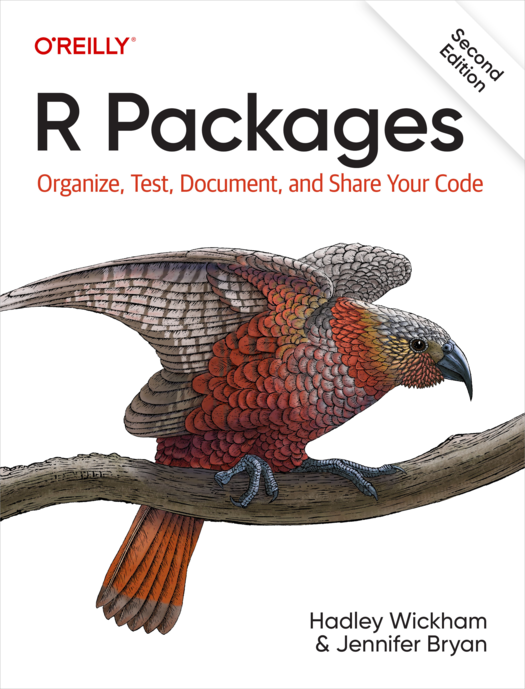
\includegraphics[width = 0.7\textwidth]{images/rpkgs-cover-2e-small.png}}
        \caption{%
          R Packages
        }
      \end{figure}%
    \end{column}
  \end{columns}

\end{frame}

\begin{frame}[standout]
  Thank you!
\end{frame}

\appendix

% \begin{frame}[allowframebreaks]{References}
%   \printbibliography[heading=none]
% \end{frame}


\end{document}

